\chapter{The South African energy sector}
The Republic of South Africa (SA) is one of the most developed country in Sub-Saharan Africa and acording to the Human Development Index (HDI) it is growing constand since the 1980's, nevertheless it counts as medium developed country \cite{UNDP2014}. Also the population and energy demand is constantly growing \cite{TheWorldBank2015,Agency2015}.

SA has also one of the strongest econemys in Africa, therefore it is accounting for about 30~\% of the primary energy consumption of the entire continent Africa in 2014 \cite{BP2015b}. 
\section{Primary energy consumption}
\begin{figure}[!b]
        \centering                
        \begin{subfigure}[b]{0.45\textwidth}
                \centering
                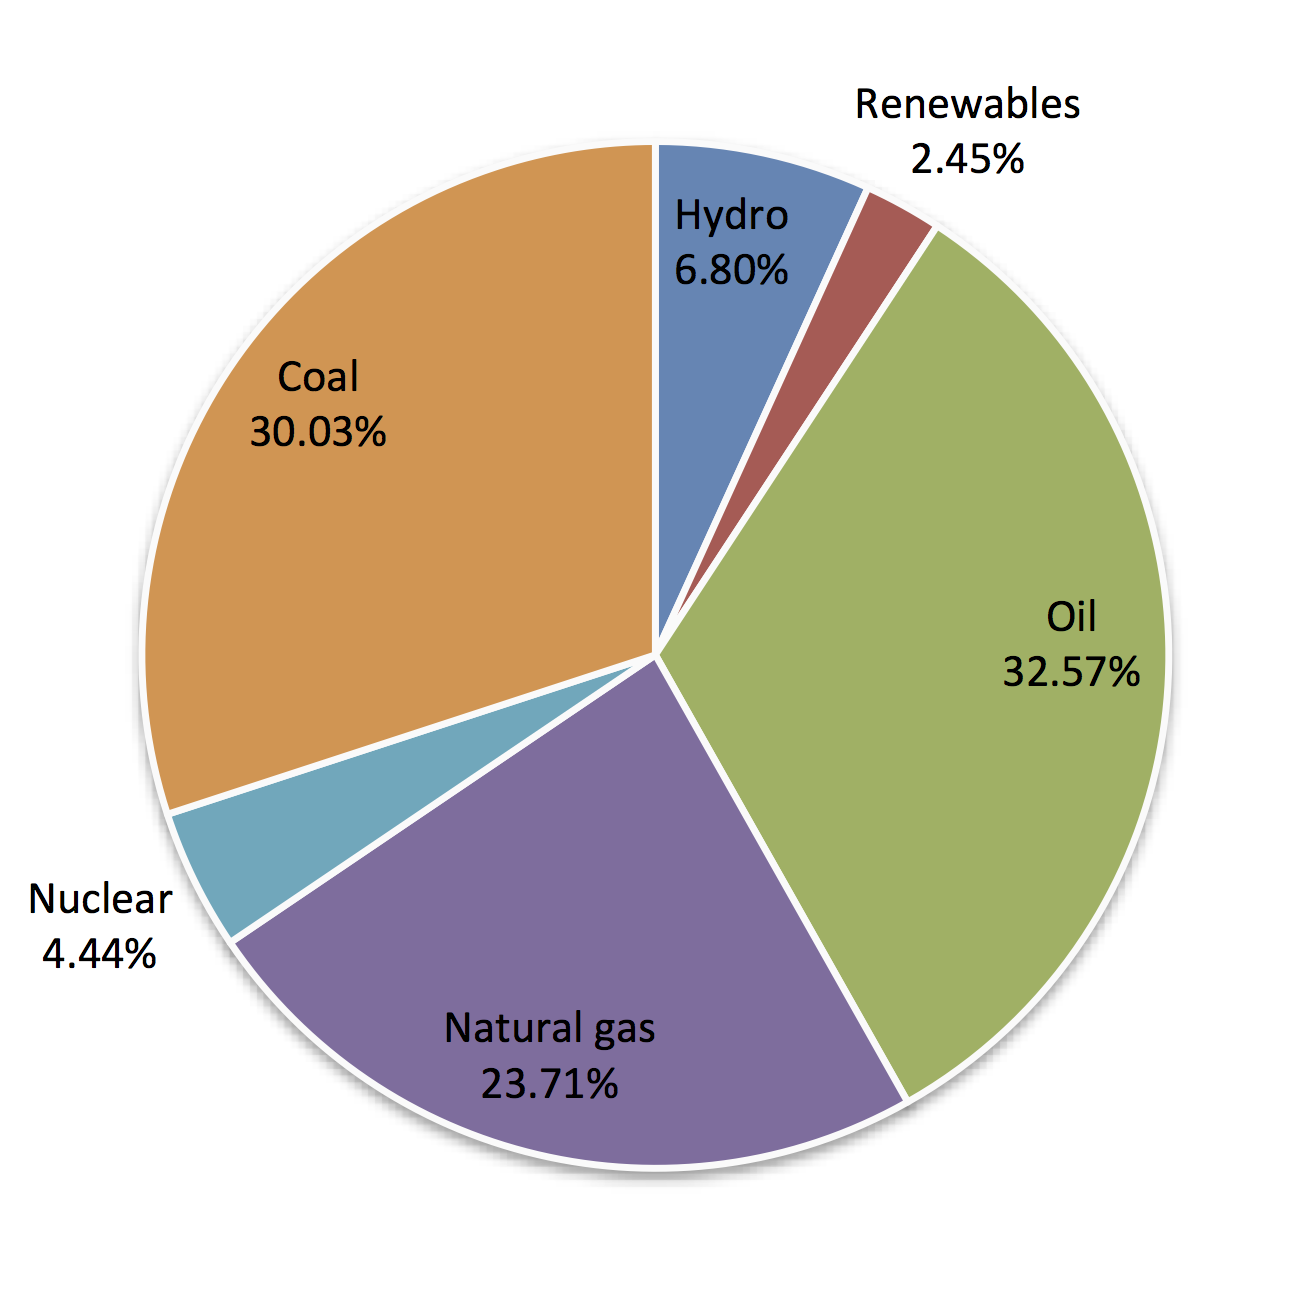
\includegraphics[width=1\textwidth]{FIG/PrimWorld}
                \caption{Worldwide allocation of primary energy consuption.}\label{PrimWorld}
        \end{subfigure}
        ~
        \begin{subfigure}[b]{0.45\textwidth}
                \centering
                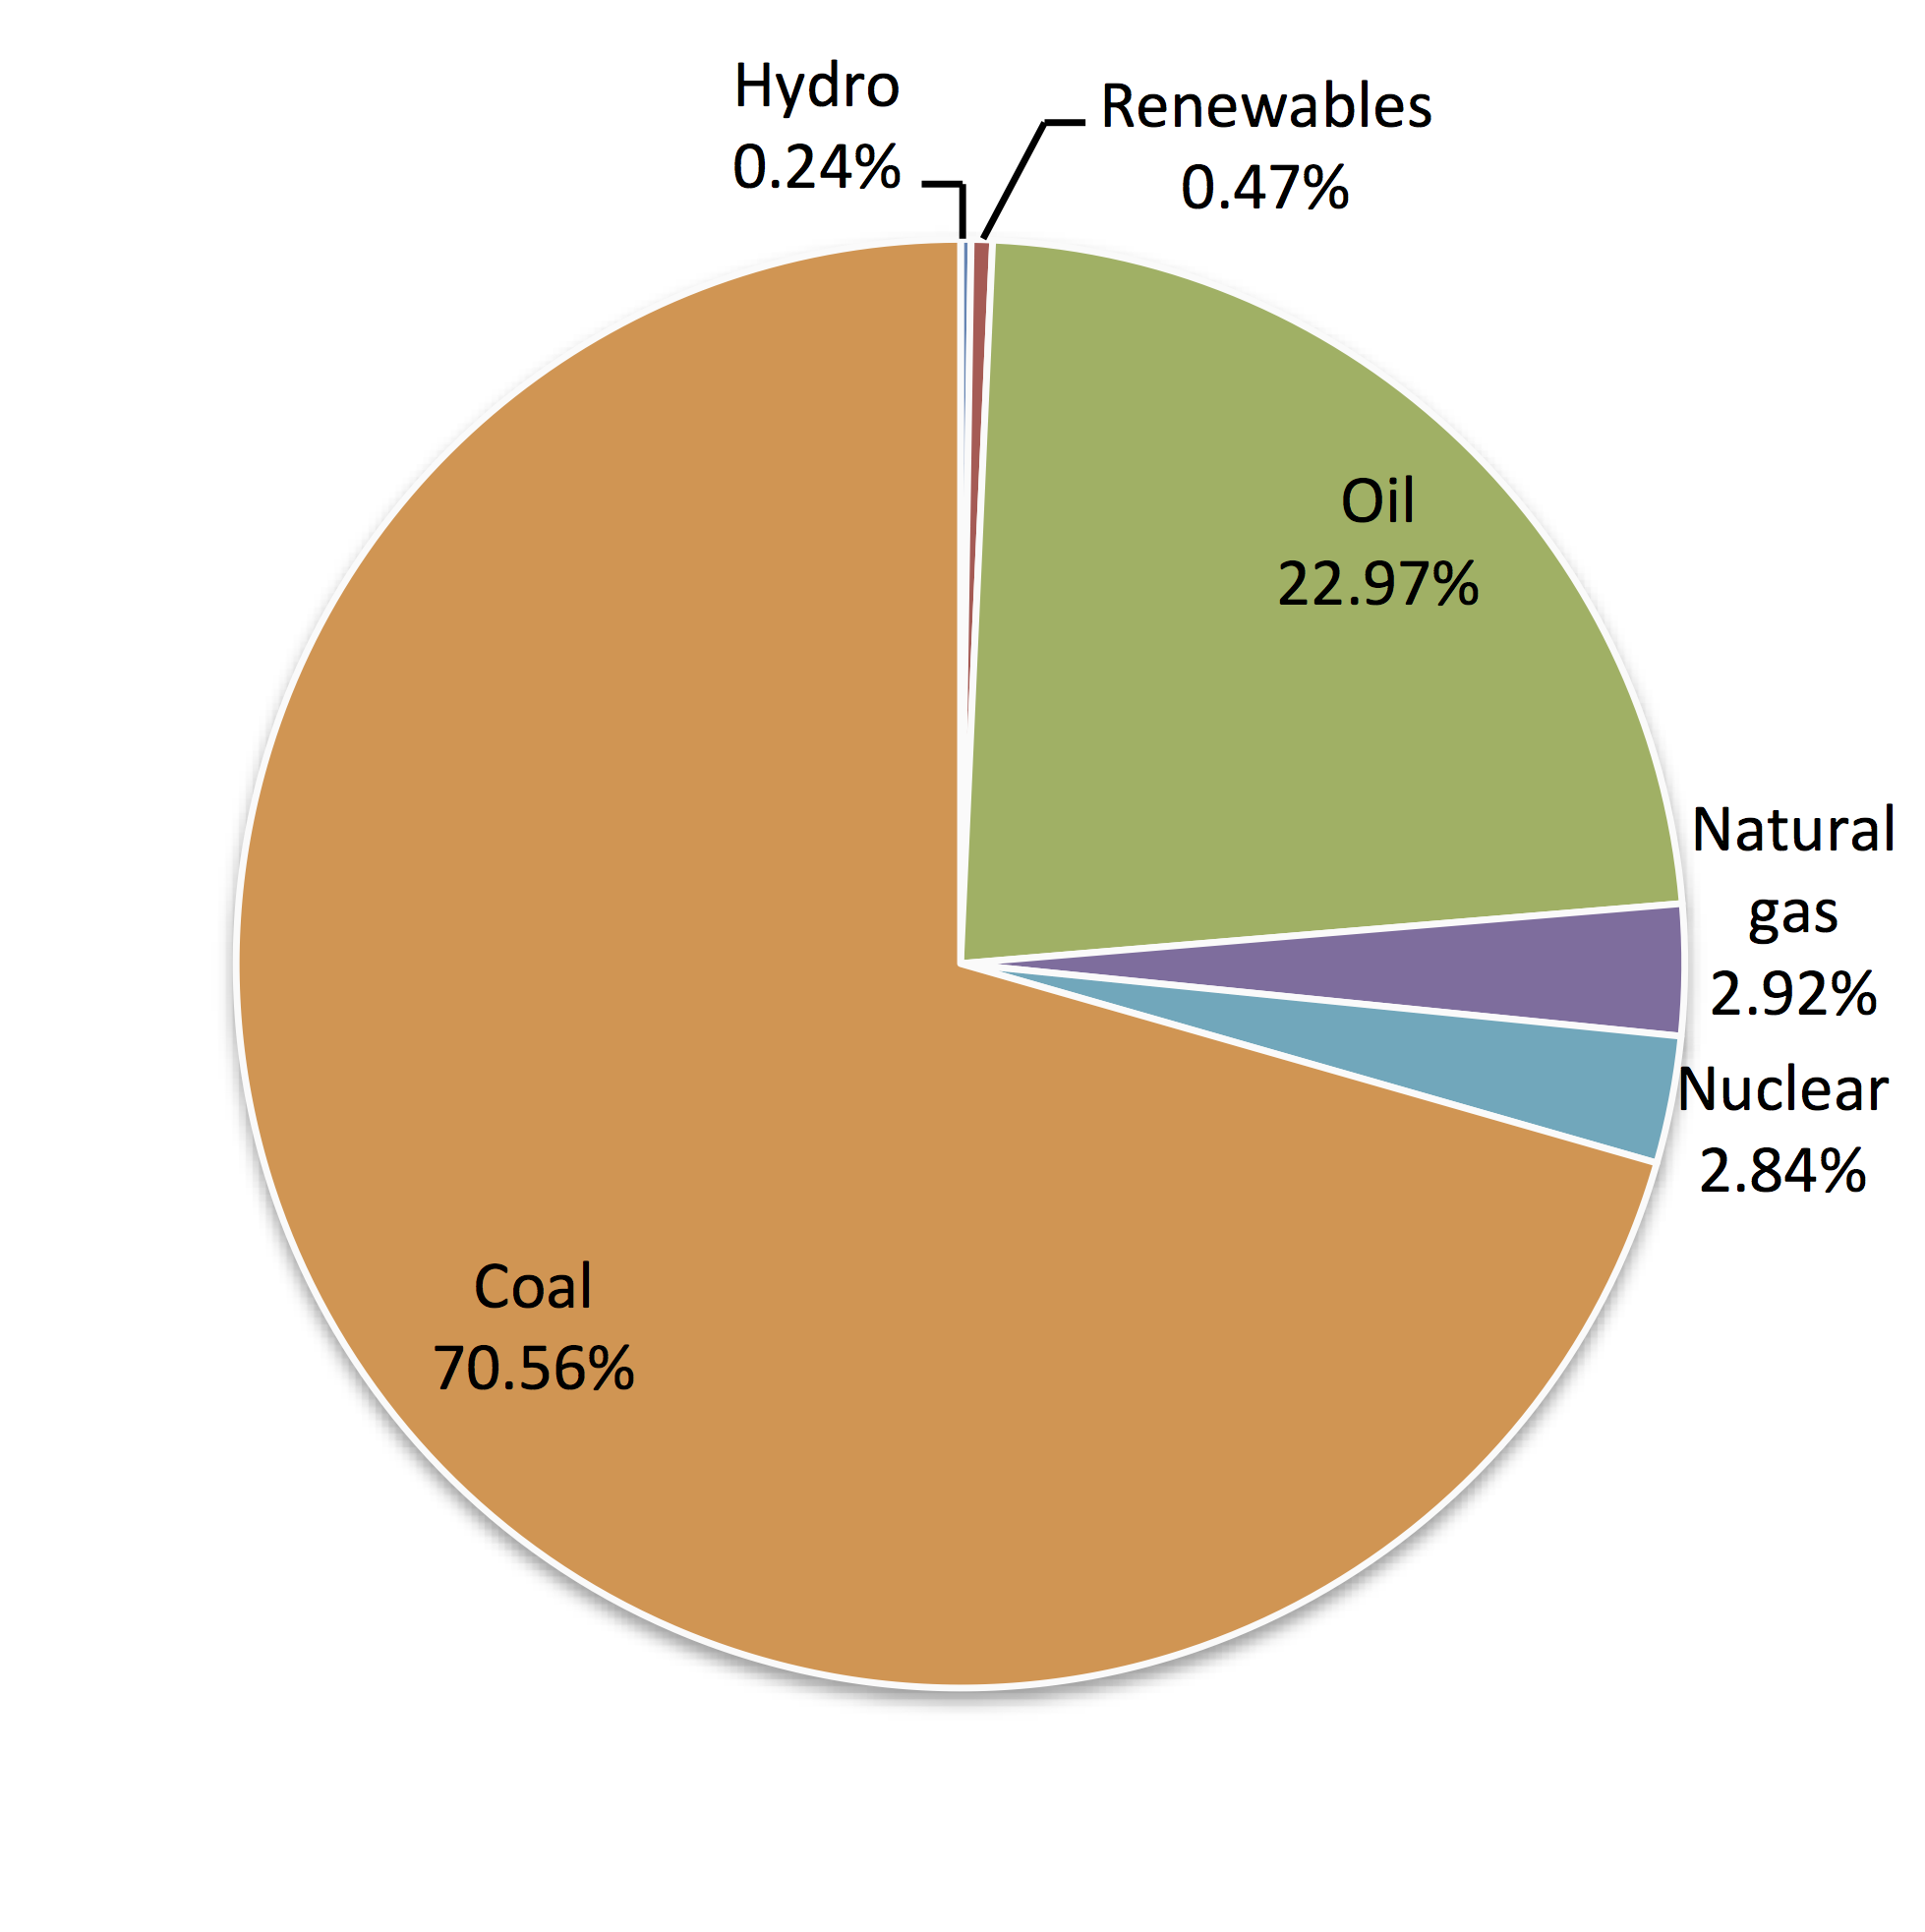
\includegraphics[width=1\textwidth]{FIG/PrimSA}
                \caption{SA's allocation of primary energy consuption.}\label{PrimSA}
        \end{subfigure}
\caption[Comparision of primary energy consumption by fuel in 2014.]{Comparision of primary energy consumption by fuel in 2014 \cite{BP2015b}.}\label{PEKreis}
\end{figure}
The primary energy consumption of SA was in 2014 about 1~473.52~TWh \cite{BP2015b}. This consumption is mainly based on fossil energy resources. More than 96~\% of the primary energy consumption was in 2014 based fossil fuels and further 2.8~\% on nuclear. Thereby is the share on primary energy consumption predominant coming from coal. Figure \ref{PEKreis} shows the primary energy mix of SA in comparision with the worldwide primary energy mix. \cite{BP2015b}

It can be seen that coal is with about 71~\% the main primary energy source. Also crude oil (23~\%) is a very important energy source for SA. Therefor is the primary energy consumption from renewable energies in SA just about 0.7~\%. Comparing to this, the global share of  renewable primary energy consumption was about 9.3~\% in 2015. But it must be said that the share on renewable energy growth almost five times from 2013 to 2014. \cite{BP2015b}

Figure \ref{PrimEnergyDevelopment} shows the growing South African primary energy consumption. Between 1965 and 2014 the annual primary energy consumption in SA has risen from 351.96~TWh up to 1~473.52~TWh. Consequently a avarage anual growing rate in primary energy consumption in SA of 8.5~\% in the past half century. \cite{BP2015c}

\begin{figure}[htbp]  
\centering
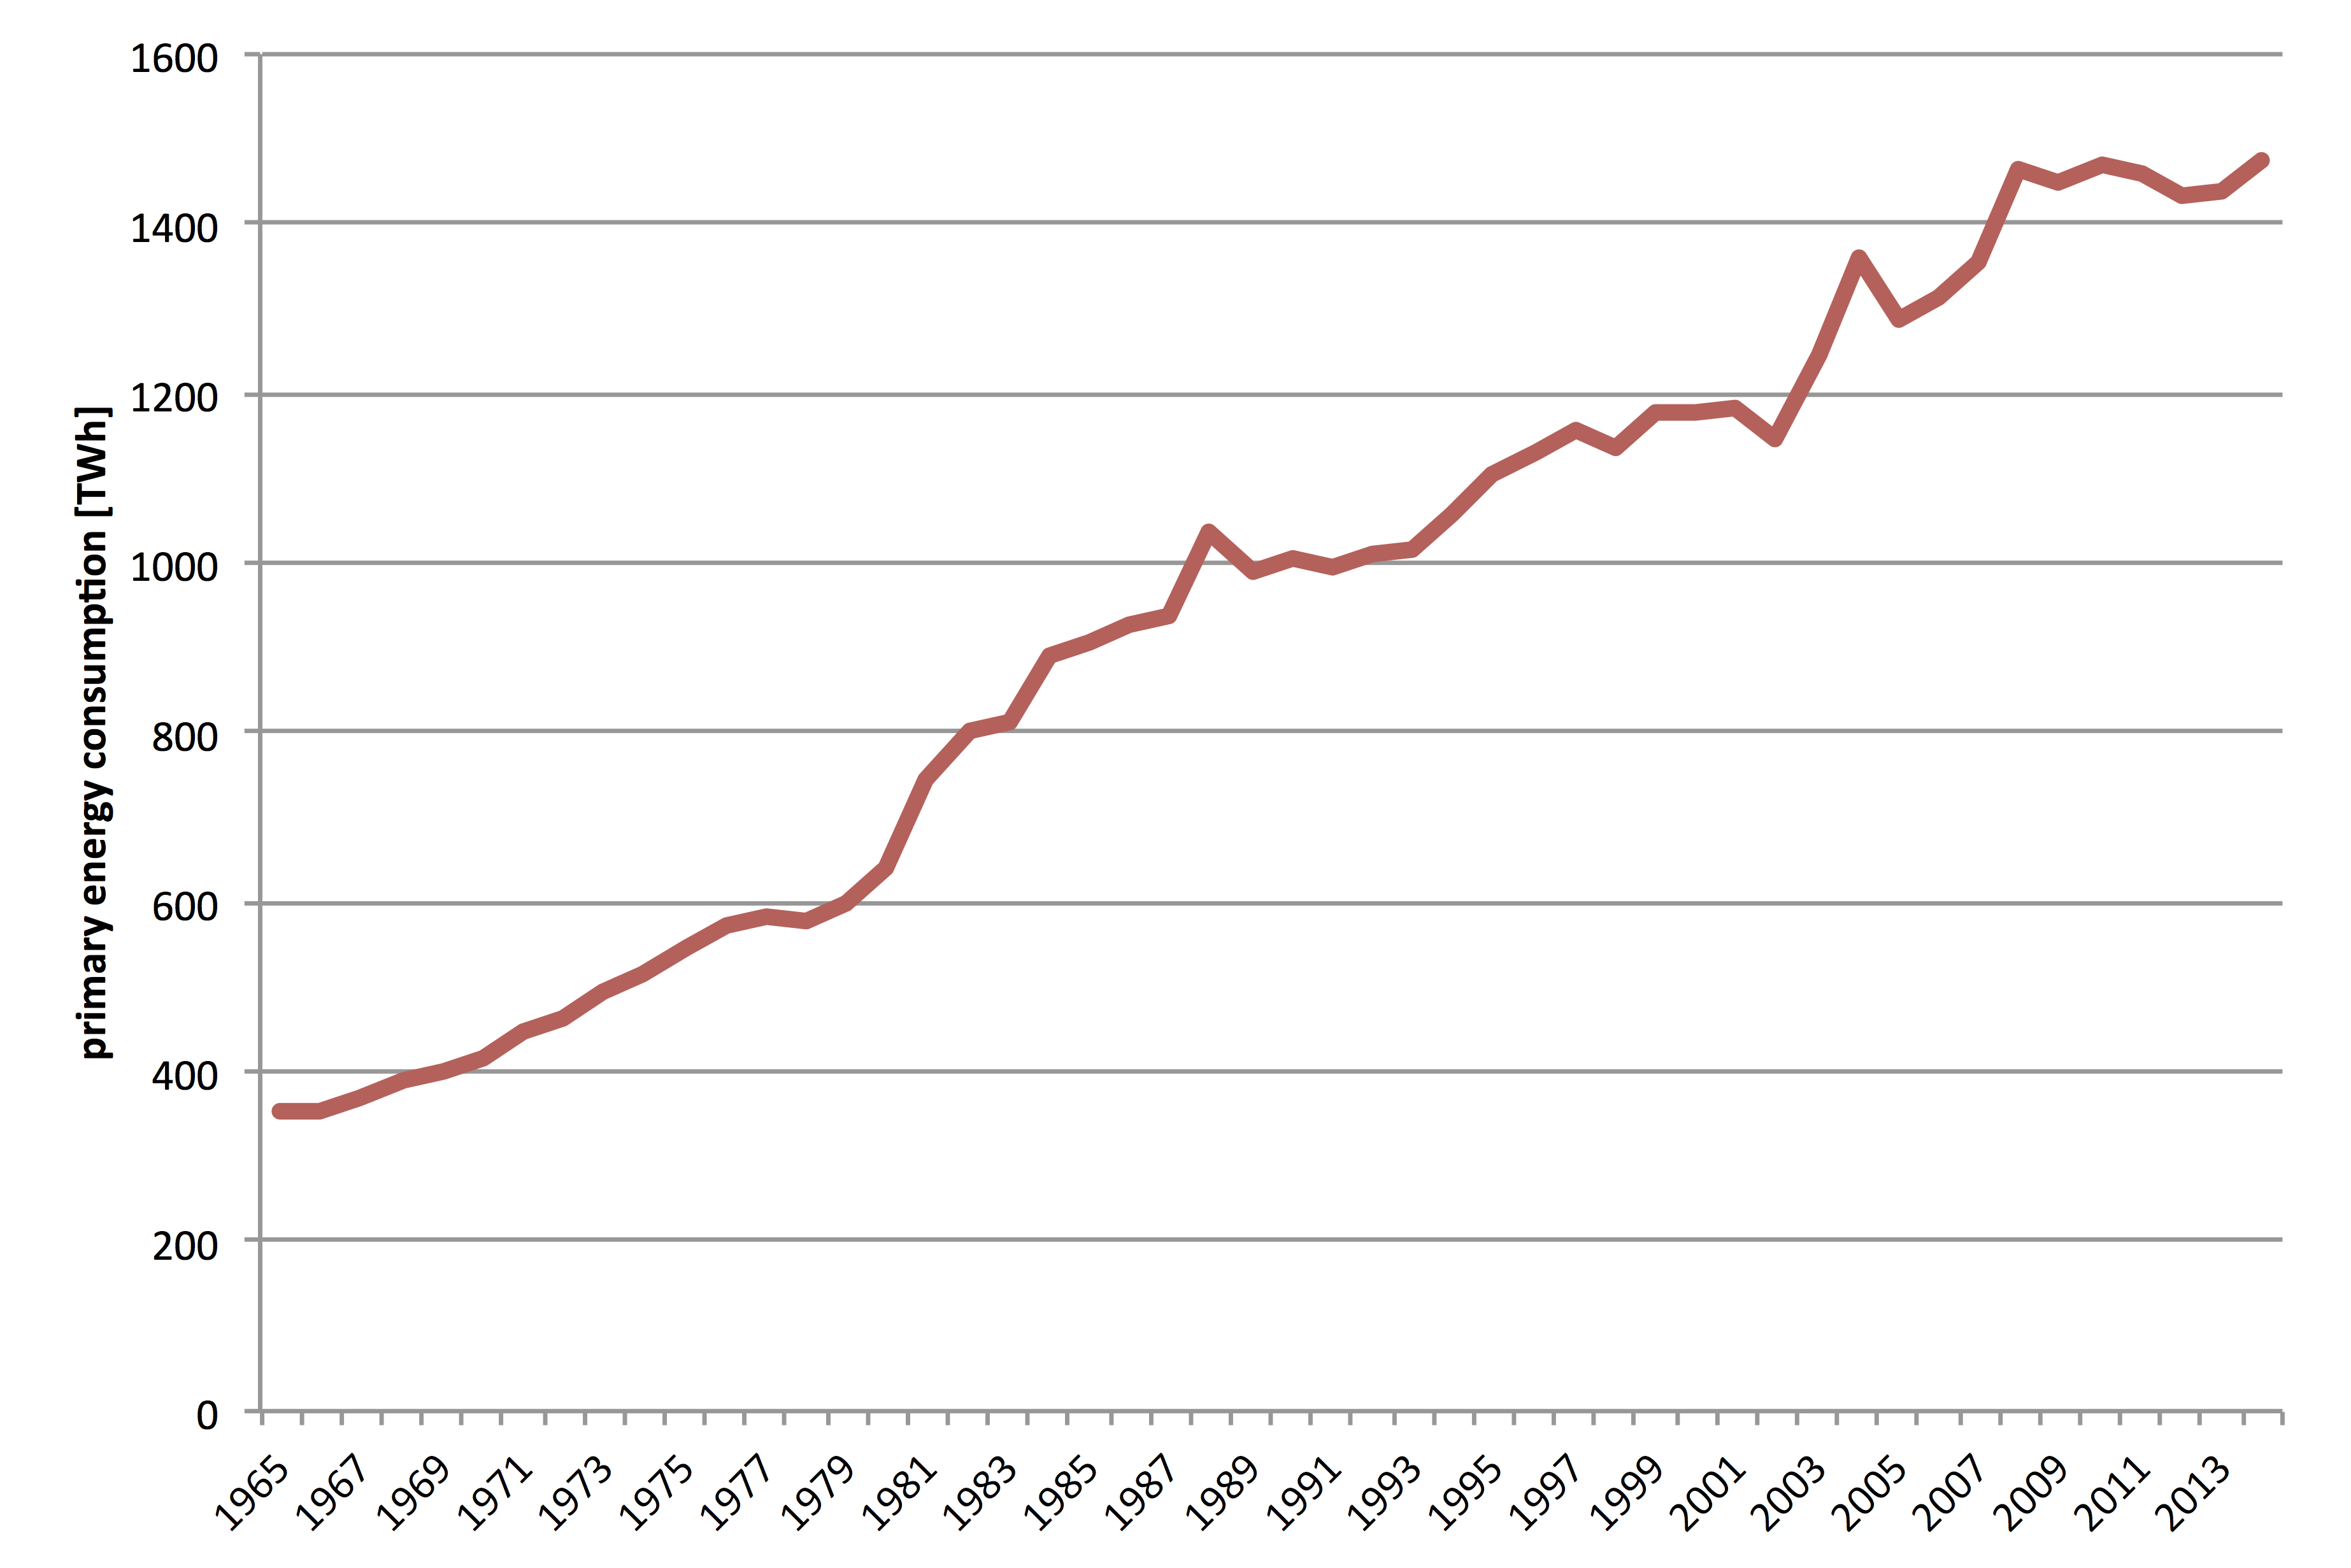
\includegraphics[width=1\linewidth]{FIG/PrimEnergyDevelopment}
\caption[Evolution of primary energy consuption of SA.]{Evolution of primary energy consuption of SA \cite{BP2015c}.}\label{PrimEnergyDevelopment}
\end{figure}
The spread in consumption of primary energy is defined by three major consumption groups, namly the industry sector with about 34.9~\%, the transport sector which consumes about 28.6~\% and other sectors with about 36.5~\%, which includes agriculture, commerce and public services, residential and non-specified consumers \cite{DepartmentofEnergy2012}. So it can be said that the sectors industy and transport are the main energy consumer in SA. 
\pagebreak
\section{Electricity supply and demand}
The electricity market in SA is regulated by the National Energy Regulator of South Africa (NERSA) in terms of the National Energy Regulatory Act from 2004. NERSA's area of responsibility includes the national grid codes, licences, provides, regulations of tariff increases and more. \cite{Eskom2015a}

SA has a fully state-owned and vertically integrated electricity supplier named Eskom (Eskom Holdings SOC Ltd.). Eskom supplies approximately 95~\% of SA's electricity and more than 45~\% of Africa \cite{EskomGenerationDivision2014}. In 2014 SA has a 1.1~\% share of the worldwide electricity consumption with a gross electricity output of 252.6~TWh \cite{BP2015c}. 92.6~\% of SA's primary energy consumption for electricity generation was based on coal fired power plants in 2013 and further 5.5~\% came by nuclear power plant \cite{Agency2015}. Therefore was Eskom in 2009 with 215.91~Mt~CO\textsubscript{2} also worldwide number five of the power companies with the highest CO\textsubscript{2} emissions \cite{CARMA2015}.

Figure~\ref{Electr} compares the South African and worldwide primary energy consumption for electricity generation in 2013. As it is shown, besides coal and nuclear based power generation makes just hydroelectric generation any significant part. \cite{Agency2015}

\begin{figure}[!htbp]
        \centering                
        \begin{subfigure}[b]{0.45\textwidth}
                \centering
                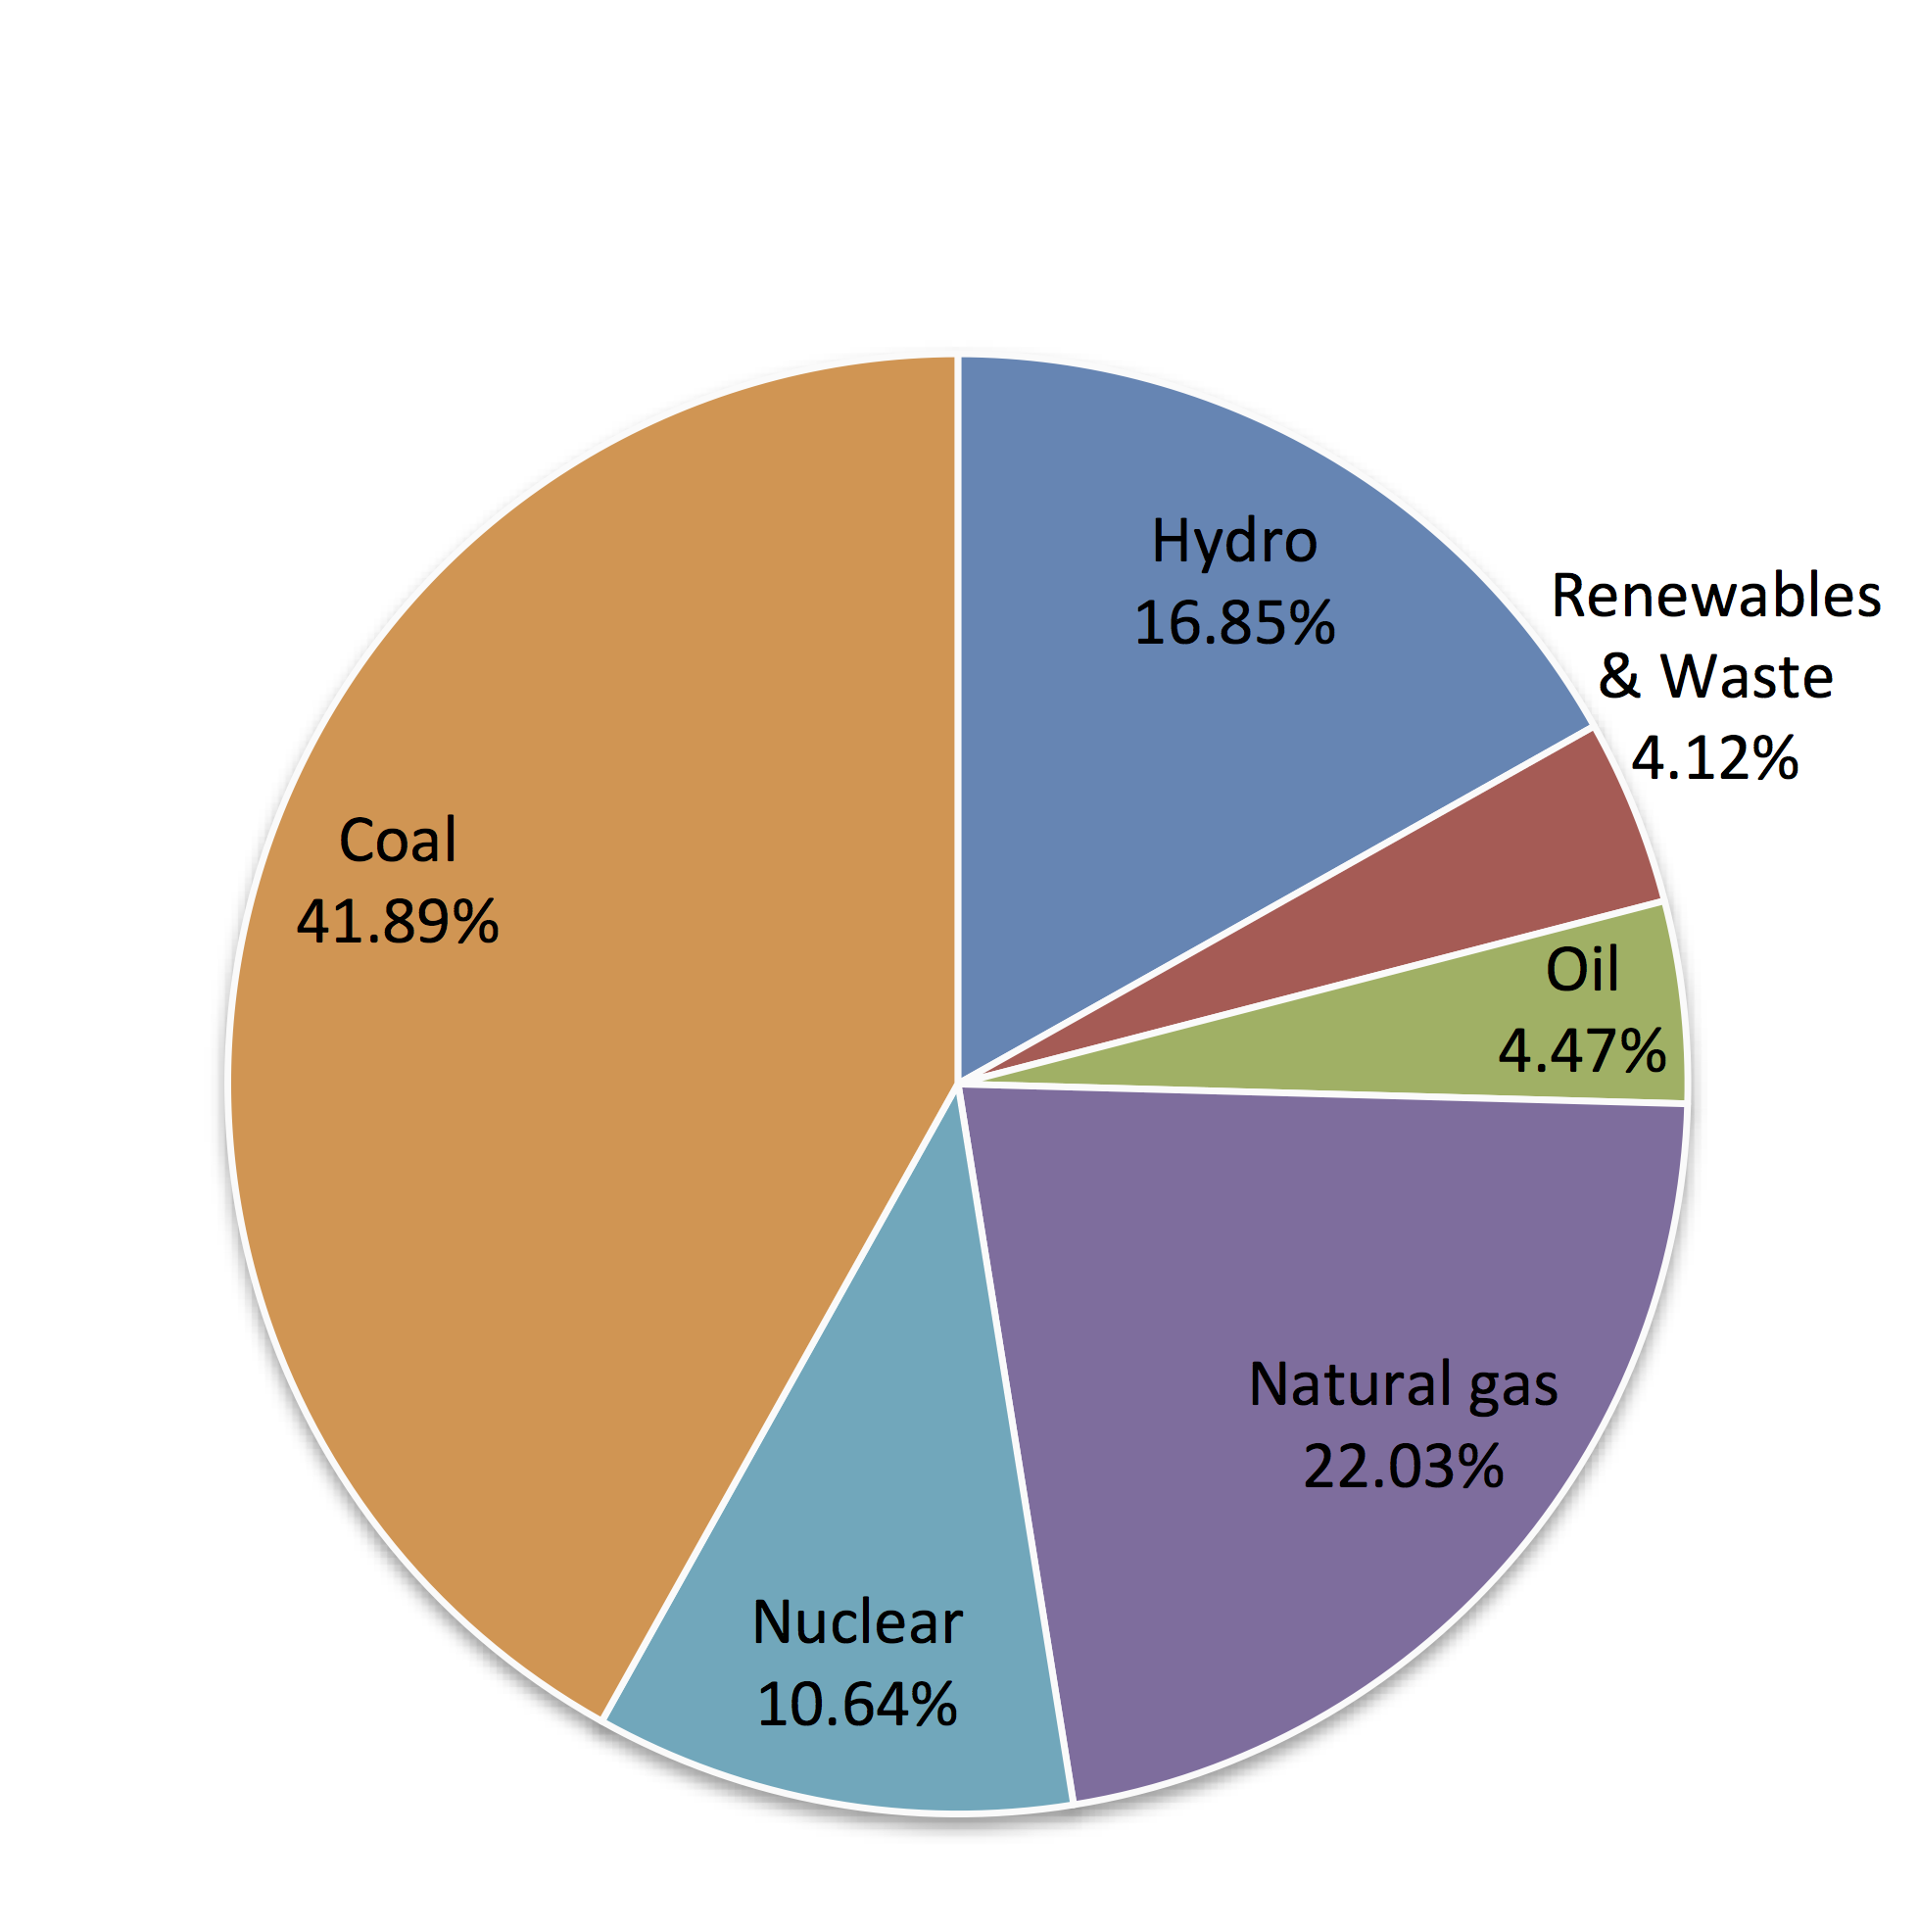
\includegraphics[width=1\textwidth]{FIG/ElectrWorld}
                \caption{World's allocation of primary energy consumption for electricity generation.}\label{ElectrWorld}
        \end{subfigure}
        ~
        \begin{subfigure}[b]{0.45\textwidth}
                \centering
                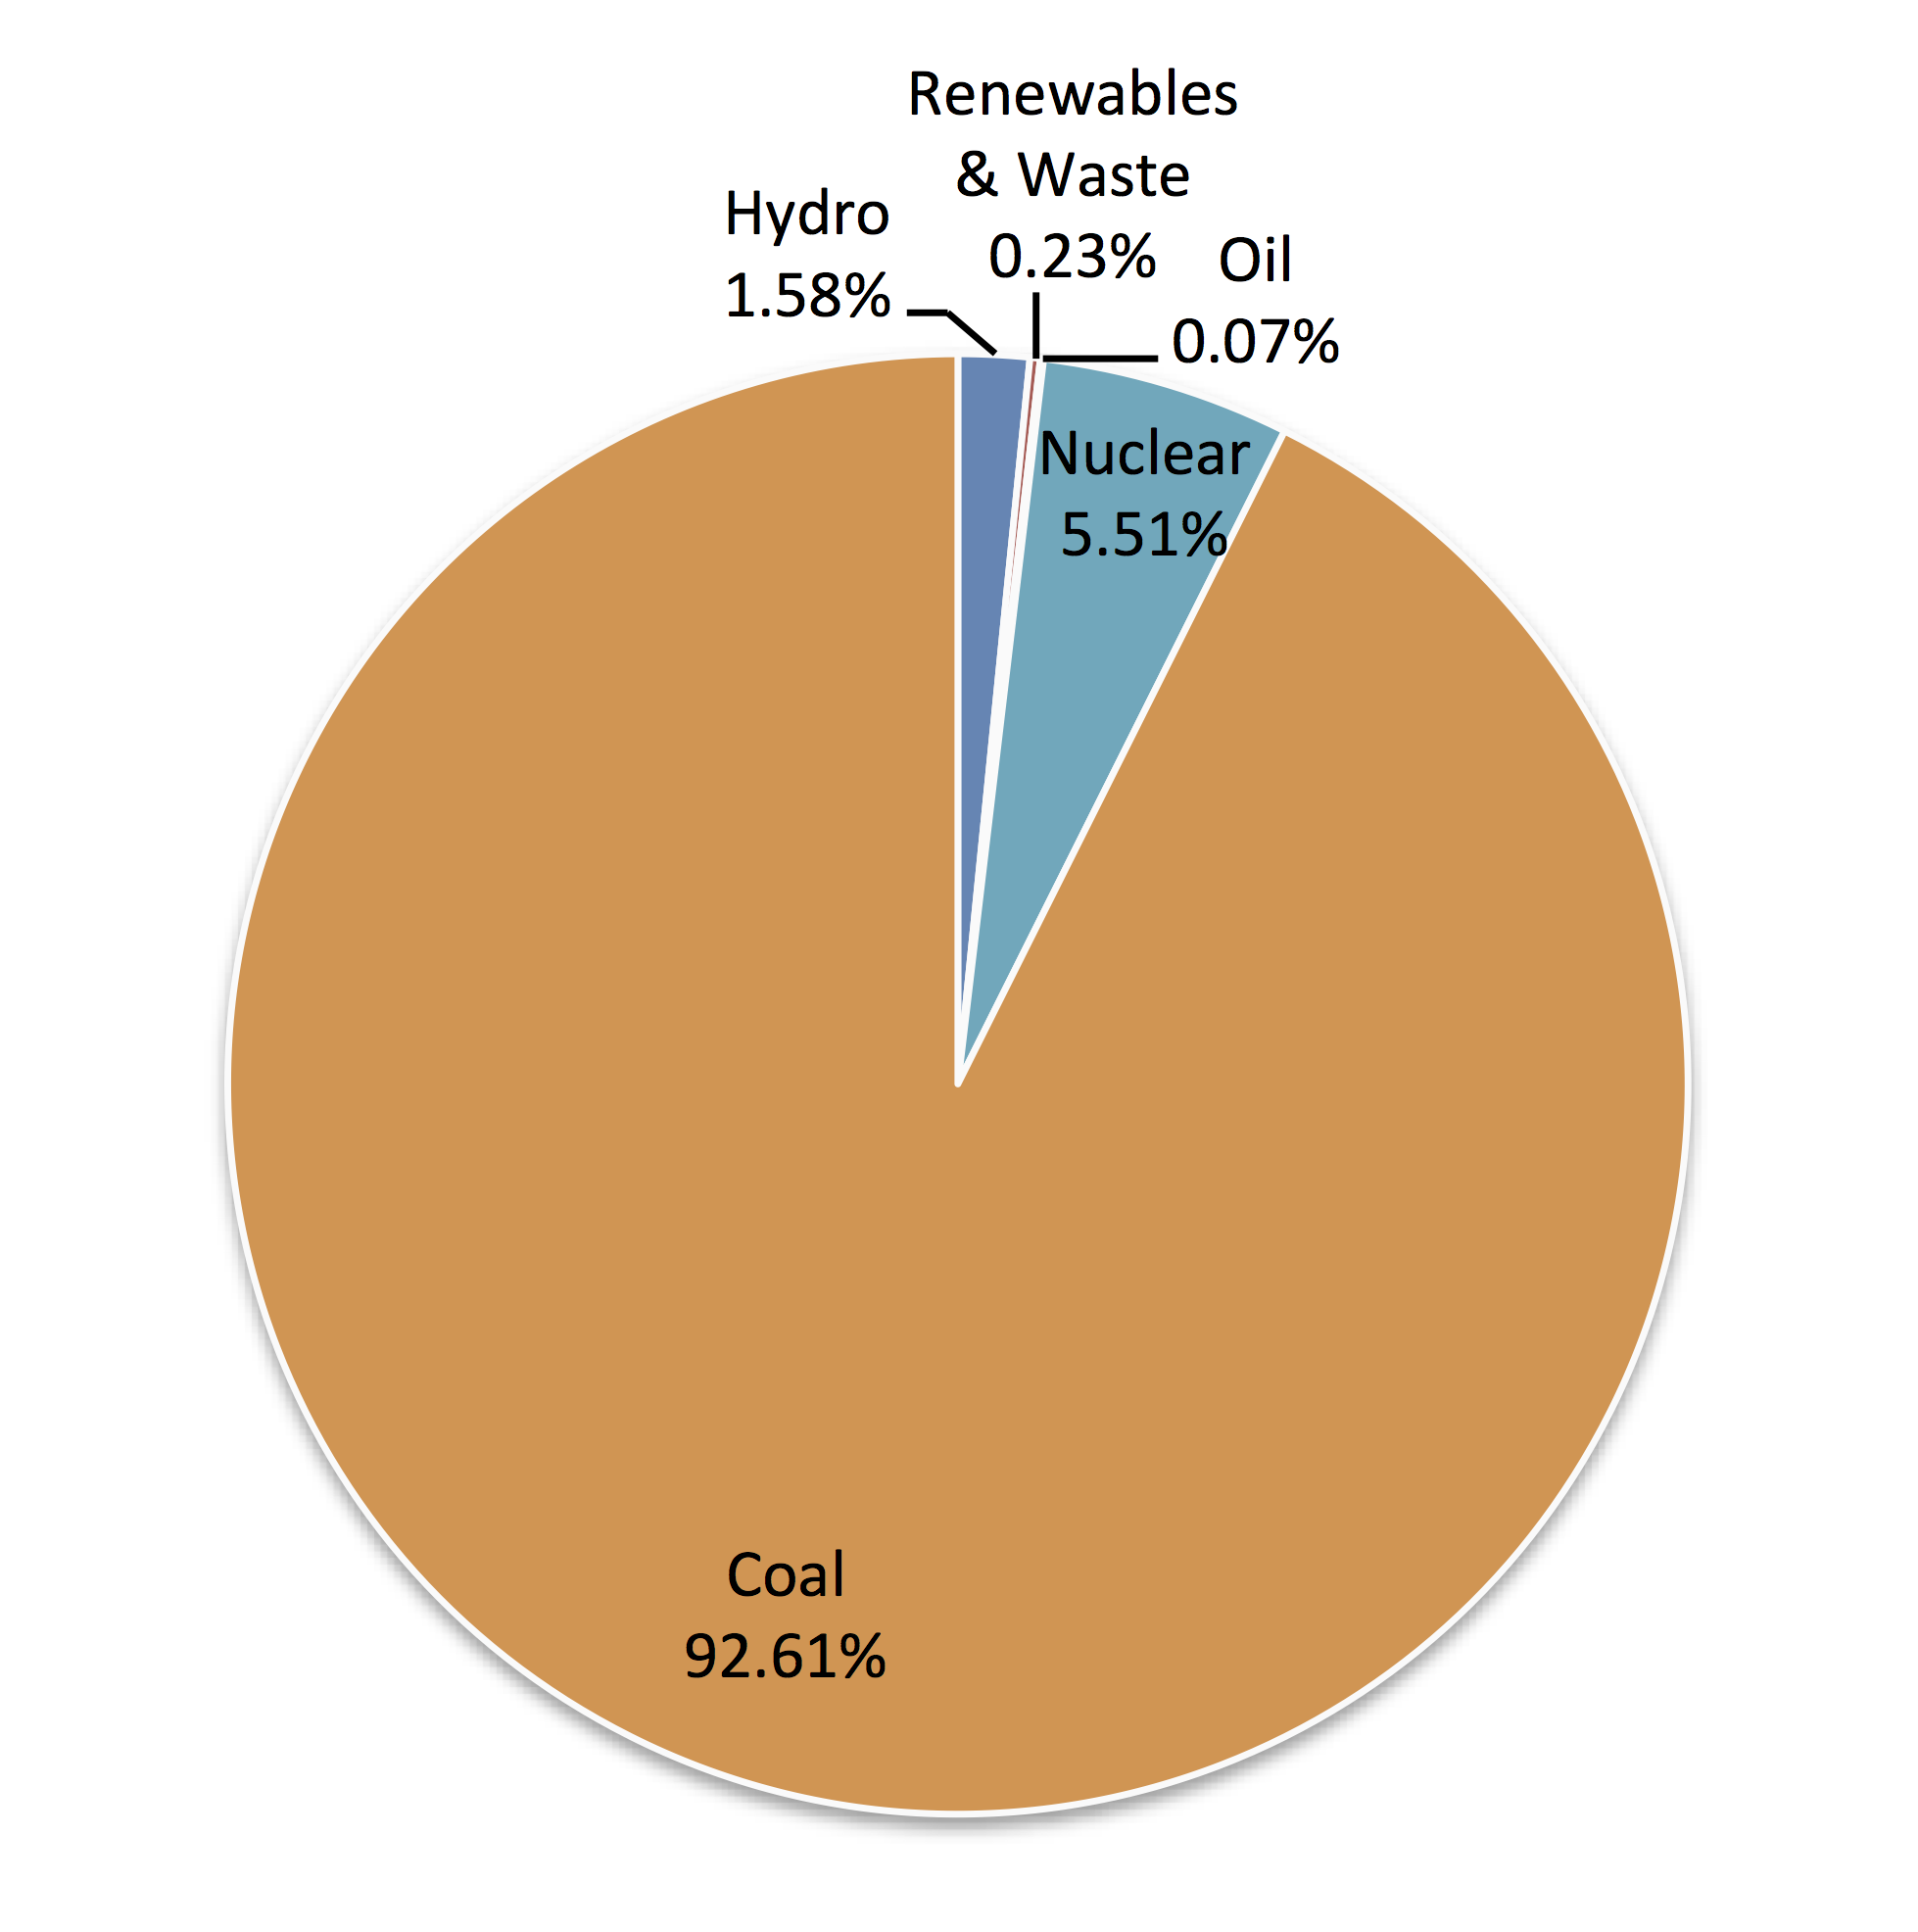
\includegraphics[width=1\textwidth]{FIG/ElectrSA}
                \caption{SA allocation of primary energy consumption for electricity generation.}\label{ElectrSA}
        \end{subfigure}
\caption[Comparision of primary energy consumption for electricity generation by fuel in 2013.]{Comparision of primary energy consumption for electricity generation by fuel in 2013 \cite{Agency2015}.}\label{Electr}
\end{figure}


\begin{figure}[htbp]  
\centering
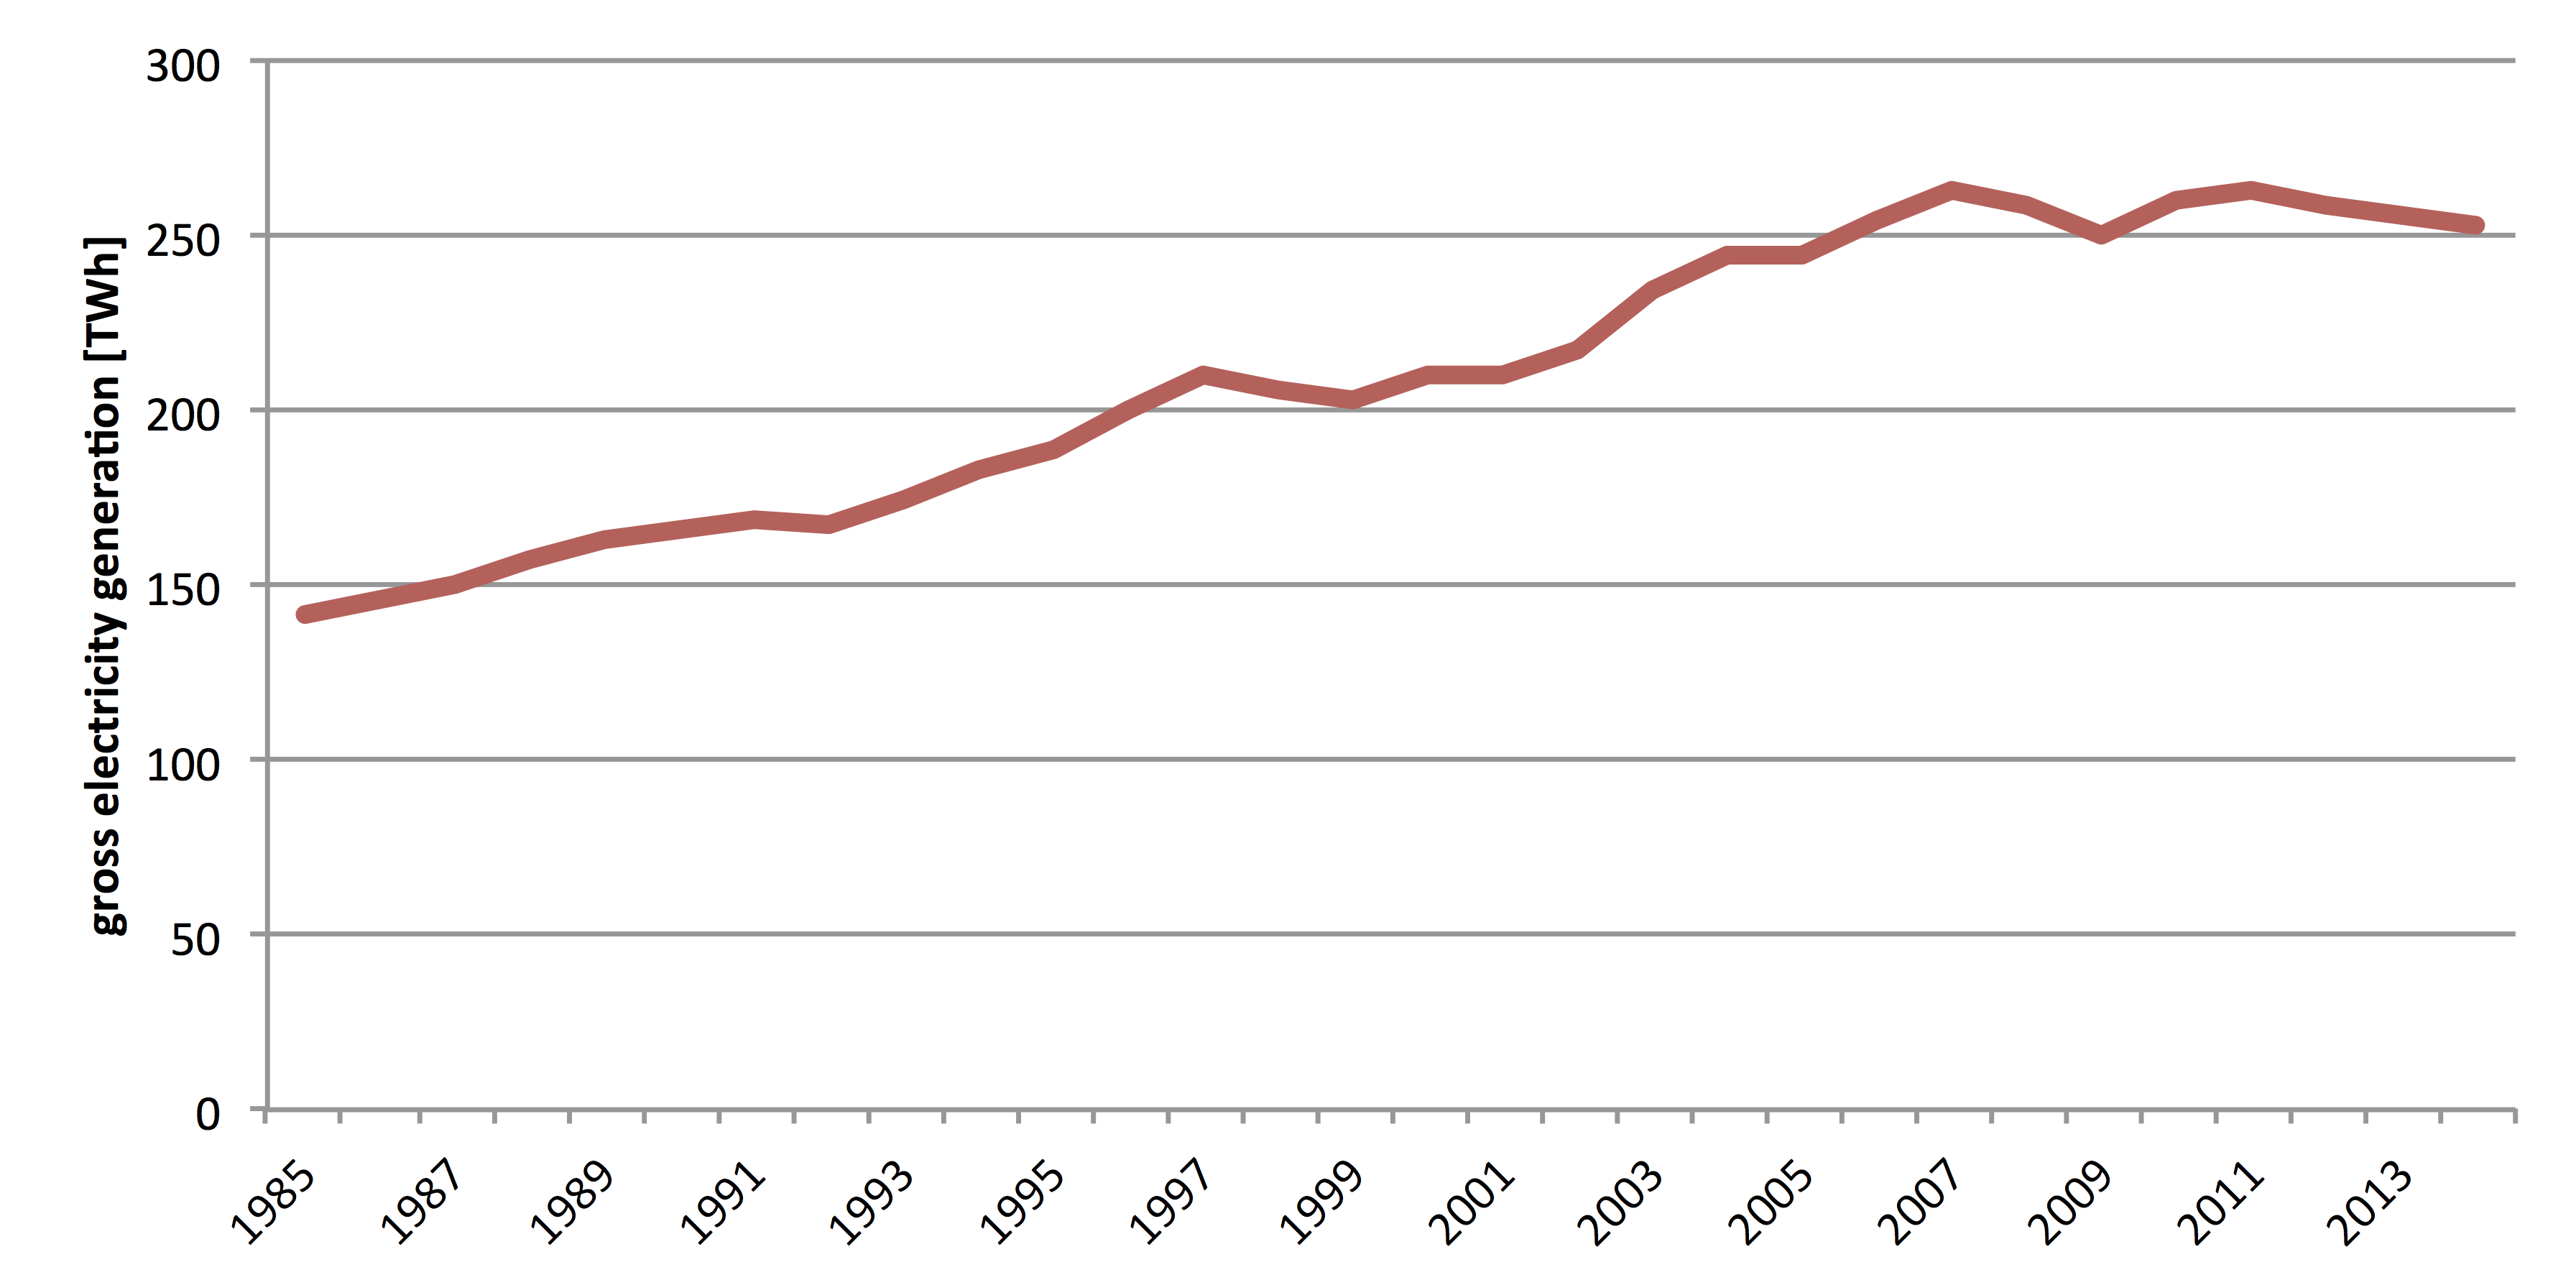
\includegraphics[width=1\linewidth]{FIG/electrGross}
\caption[Evolution of gross electricity generation in SA.]{Evolution of gross electricity generation in SA \cite{BP2015c}.}\label{electrGross}
\end{figure}

The final electricity consumption in SA was about 197~092~GWh in 2012. The final consumption consist also three main consumers. The largest consumer group with about 59.5~\% are industrial consumers, followed by residential consumers (19.7~\%) and commercial and public services (14.3~\%). The complete electricity flow is shown in Annexure I, Part A, Table \ref{tab1}, on page \pageref{tab1}. \cite{Agency2015}

\subsection{Rising energy consumption and security of supply}

\begin{figure}[!h] % Monthly Reserve
\centering
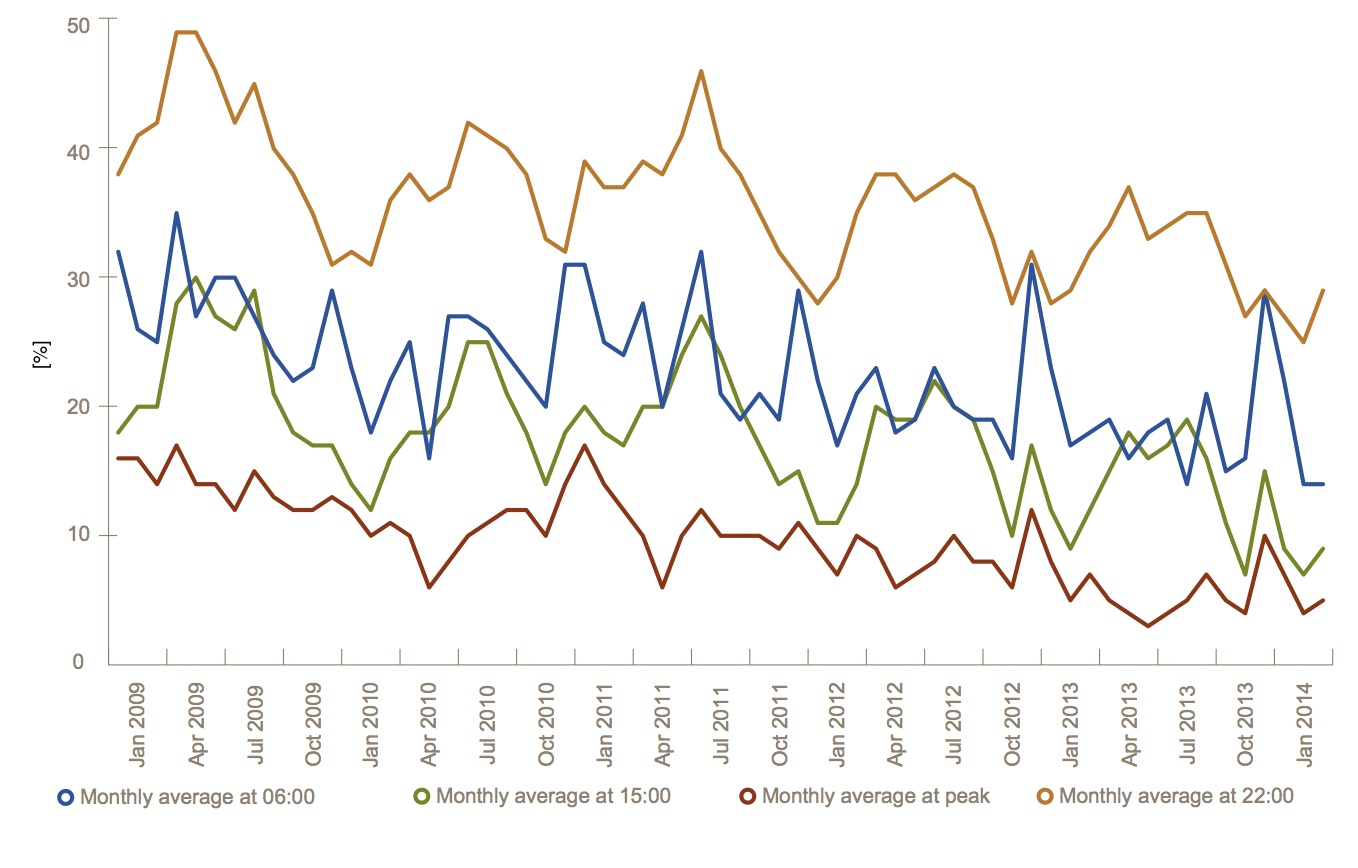
\includegraphics[width=0.9\linewidth]{FIG/AveragemonthlySA}
\caption[Average monthly \% operating reserves.]{Average monthly \% operating reserves\cite{Eskom2014}.}\label{Abb1}
\end{figure}


\begin{figure}[!h] % Demand growth
\centering
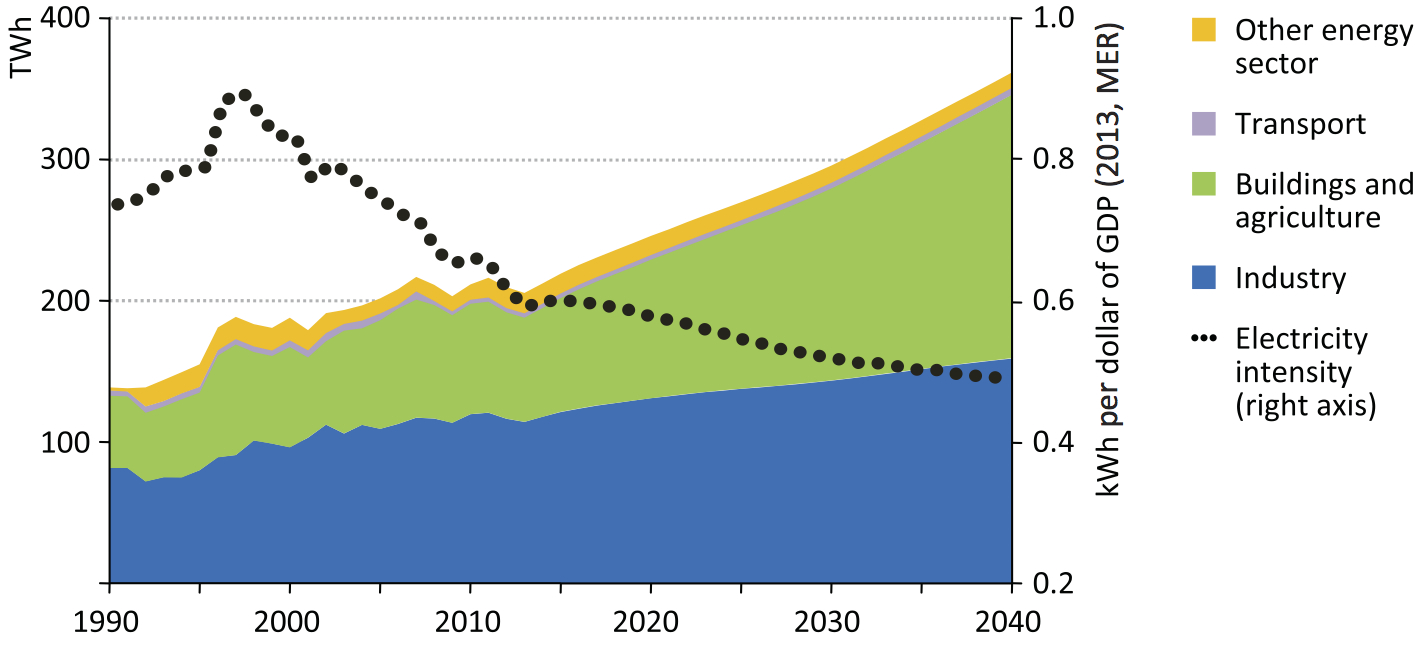
\includegraphics[width=0.9\linewidth]{FIG/SA_Electricity_demand_growth}
\caption[Electricity demand growth by sector in South Africa in the New Policies Scenario.]{Electricity demand growth by sector in South Africa in the New Policies Scenario \cite{IEA2014f}.}\label{Abb1}
\end{figure}

\subsection{Structure of power distribution}
Kilometerlängen, Verluste im Netz \cite{Eskom2014a}

SA's power supply system is controlled to a frequency of 50Hz.

On mainland sub-Saharan Africa, SA has with around 85~\% the highest electrification rate. About 11~\% of households don't have access to electricity and a further 4~\% rely on illegal access (non-paying) or obtain access informally (from one household to another but paying). \cite{IEA2014f}

\begin{figure}[htbp]
\centering
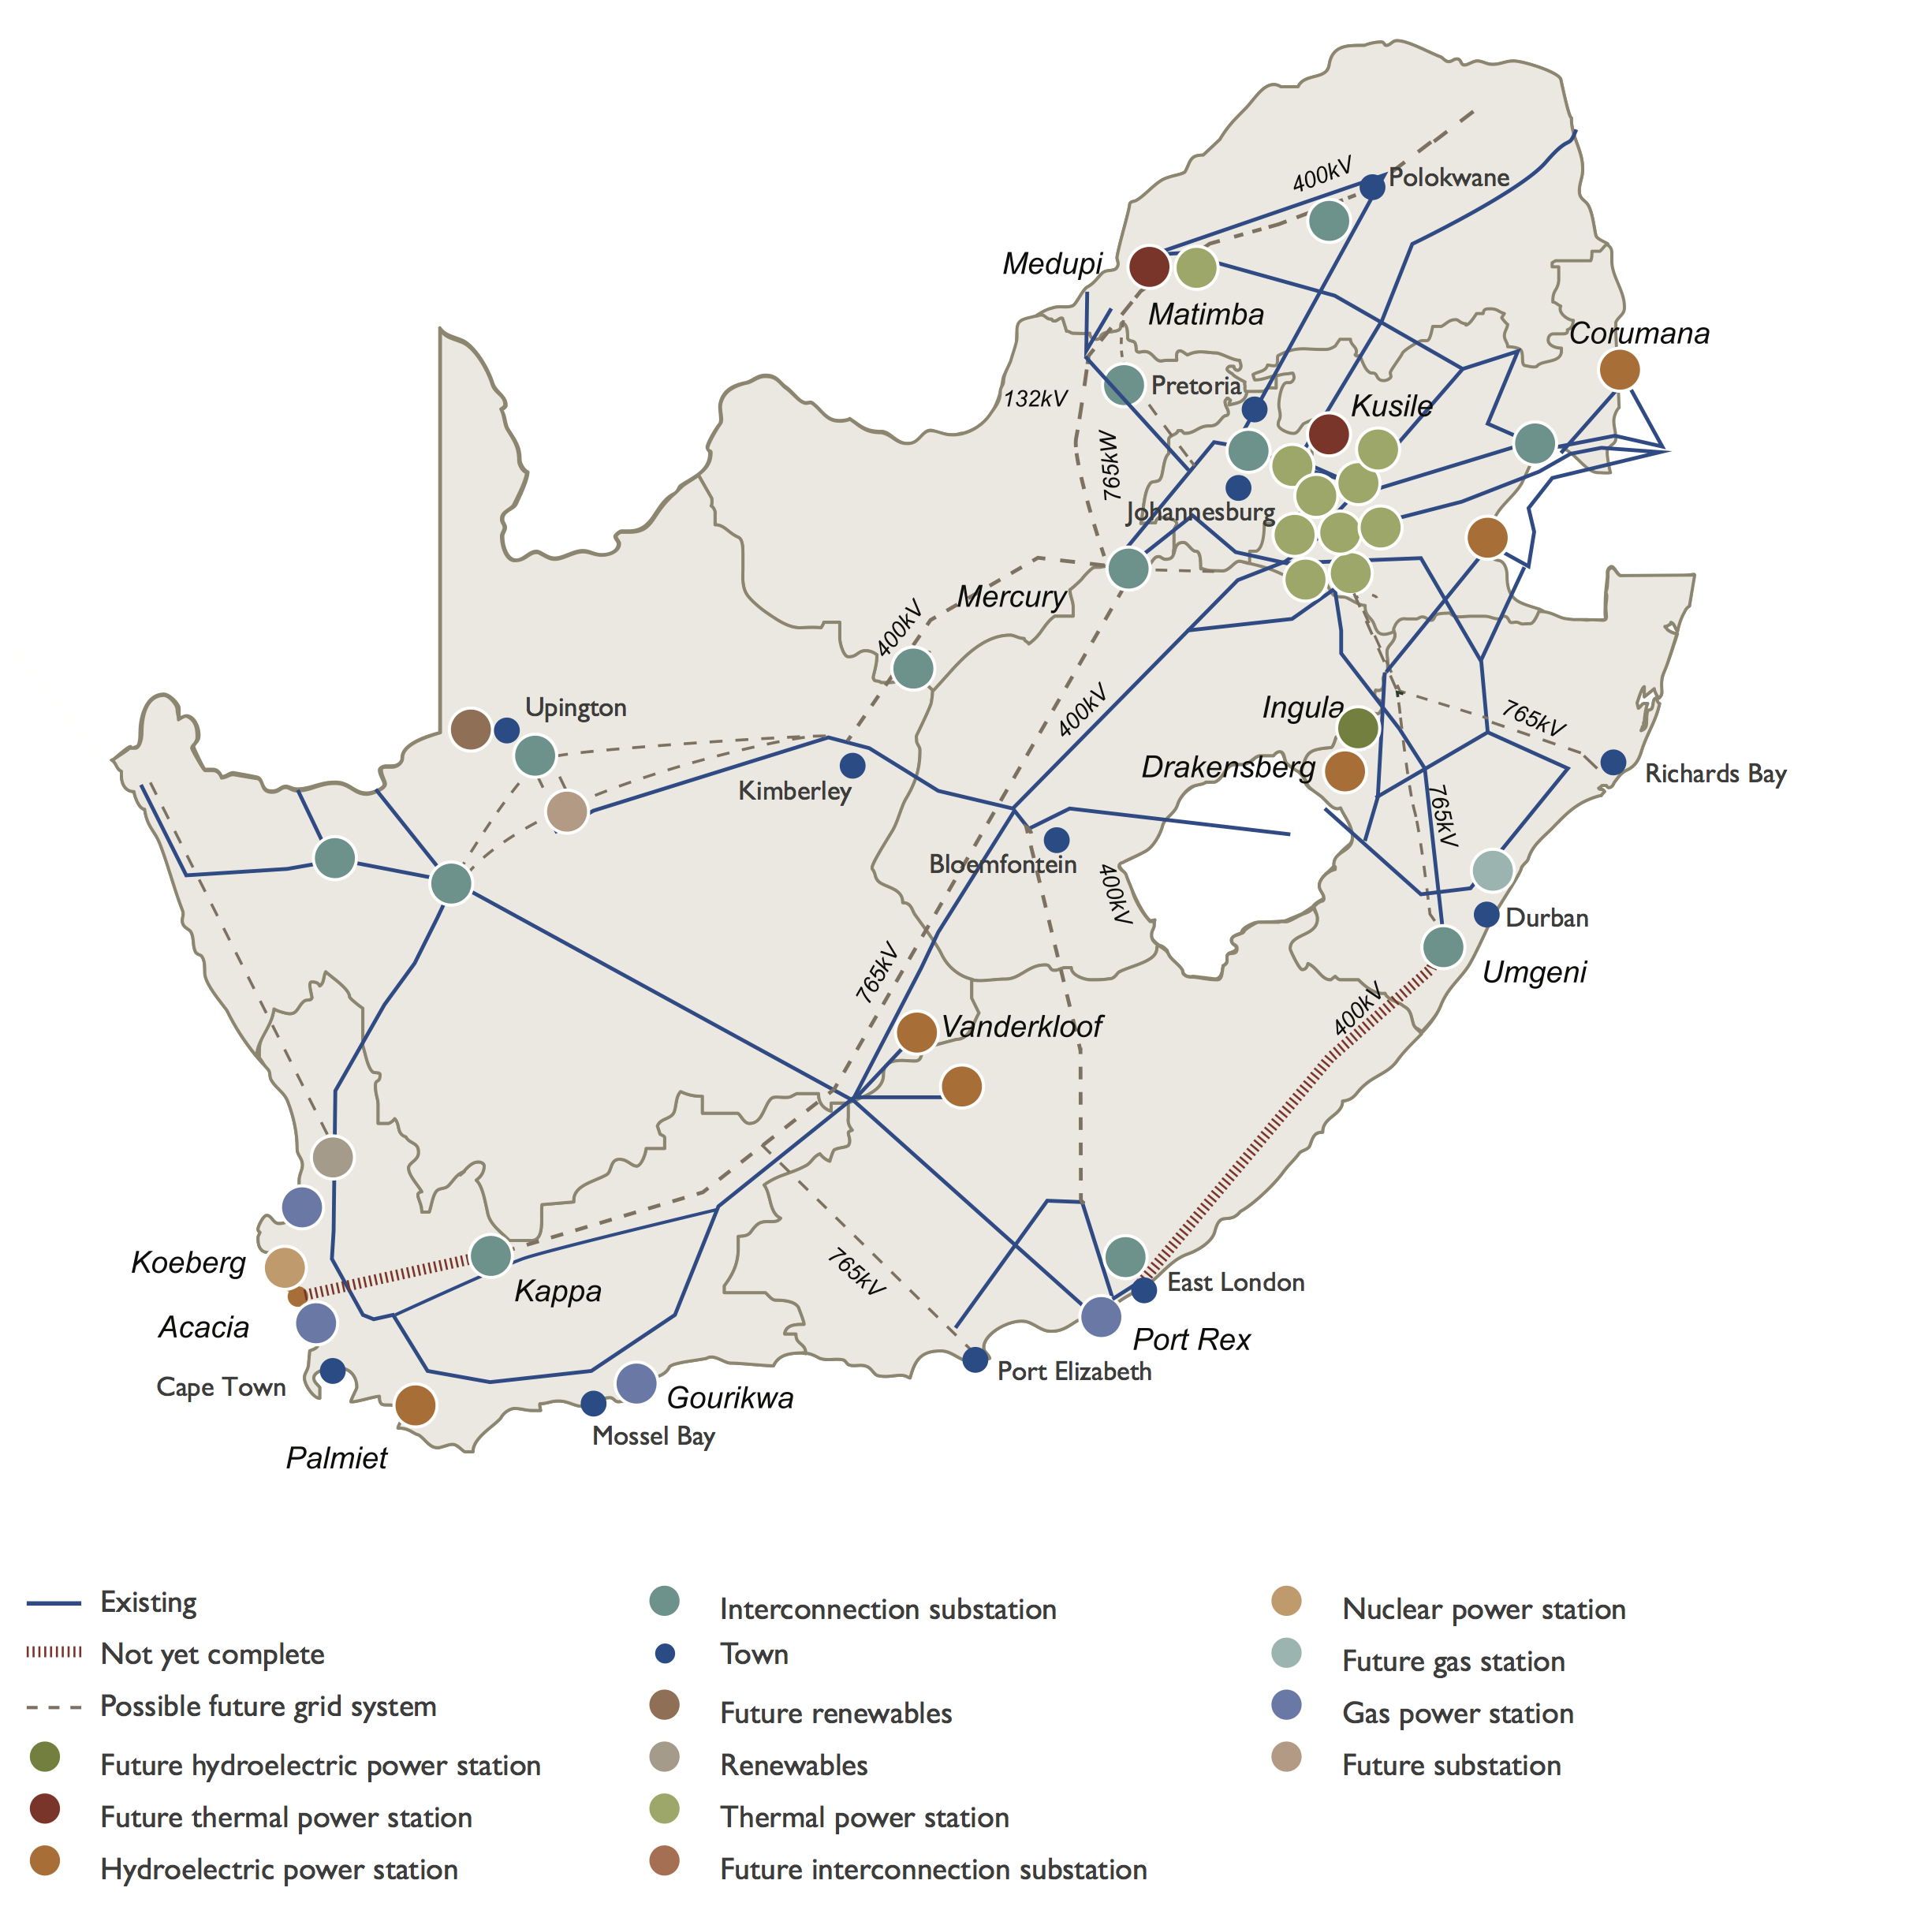
\includegraphics[width=1\linewidth]{FIG/transmissionprojekts}
\caption[Eskom’s transmission projects as at 31 March 2015.]{Eskom’s transmission projects as at 31 March 2015 \cite{Eskom2015a}.}\label{transmissionprojekts}
\end{figure}

http://integratedreport.eskom.co.za/supplementary/app-transmission.php

\section{Renewable energy potential in South Africa}

\subsection{Energy outlook for South Africa}
Development of a Renewable Energy Power Supply Outlook 2015 for the Republic of South Africa
Achieved by Sebastian Giglmayr, BSc
\cite{Giglmayr2013}

\subsection{Government Incentives}

\section{Chapter summary}
\pagebreak
